% !TEX root = ../VPJ.tex

\chapter{Grundlagen und Konzepte}
\label{sec:Grundlagen}

In diesem Kapitel werden einige Grundlagen erläutert, die zum Verständnis der späteren Kapitel der Arbeit beitragen. 

\section{Qt}

Qt ist eine plattformübergreifende Anwendungsentwicklungsumgebung für Desktopanwendungen, eingebettete und mobile Systeme. Unterstützt werden unter anderem Linux, OS X,  Windows, Android, iOS, BlackBerry oder Sailfish OS. 

Die Umgebung ist in C++ geschrieben, weshalb vorwiegend in dieser Sprache programmiert wird. Eine Besonderheit an Qt ist die Benutzung eines Signal-Slot-Systems. 

Ähnlich anderen Entwicklungsumgebungen bietet Qt mit einem implementierten Designer Möglichkeiten zur GUI-Programmierung mit vorgefertigten Widgets (vgl. \cite{qt_allgemein}).

Die nächsten Abschnitte zeigen einige Besonderheiten von Qt und Konzepte, die in der Ausarbeitung des Projekts verwendet wurden. 

\subsection{Eventbasiertes System}
\label{sec:Eventbasiert}

Innerhalb von Qt werden Signale und Slots zur Kommunikation zwischen Objekten genutzt. Das Signal-Slot Konzept ersetzt das in anderen Umgebungen verwendete Callback-System, welches beispielsweise in Eclipse bei der Java-Programmierung oder in Visual Studio mit C\# verwendet wird. 

\begin{figure}[htb]
    \centering
    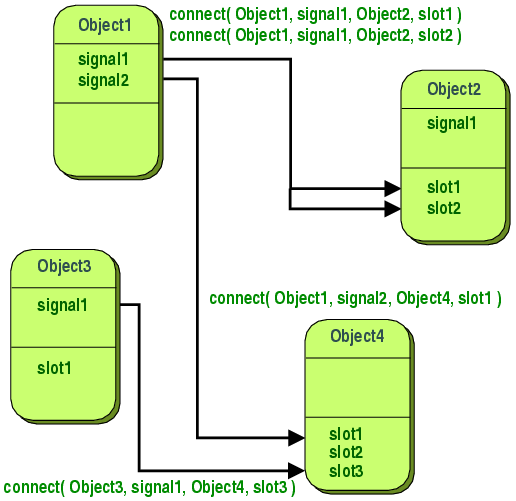
\includegraphics[width=0.5\textwidth]{Abbildungen/signalslots.png}
    \caption[Signale und Slots in Qt \newline Quelle: \textit{https://doc.qt.io/qt-5/signalsandslots.html}]{Signale und Slots in Qt}		
    \label{fig:signalslots}
\end{figure}

In Abbildung \ref{fig:signalslots} ist das Konzept visuell dargestellt. Ein Signal wird immer dann emittiert, wenn ein bestimmtes Event auftritt. Die in Qt verwendeten Widgets stellen bereits viele dieser Signale bereit, können jedoch um eigene ergänzt werden. 

Das Gegenstück zu den Signalen sind Slots, welche als Antwort auf ein Signal aufgerufen wird. Es können beliebig viele Signale an einen Slot gebunden werden. Es ist ebenfalls möglich Signale direkt an weitere Signale zu binden. 

Ein Slot kann wie eine normale Funktion auch mittels Funktionsaufruf verwendet werden.  

Nähere Informationen zu diesem Konzept, zu Signalen und zu Slots können der Quelle \cite{qt_signalslot} entnommen werden. 

Um Signale und Slots zu verbinden werden verschiedene Möglichkeiten bereitgestellt. In dieser Arbeit wurde hauptsächlich mit der connect() Funktion gearbeitet, die von jeder Klasse, die von QObject erbt, bereitgestellt wird. 

\begin{lstlisting}[frame=single, breaklines=true, numbers=left, stepnumber=2, firstnumber=1, numberstyle = \tiny, caption=Connect Signals and Slots ,label=lst:Connect]
QObject::connect(const QObject *sender, const char *signal, const QObject *receiver, const char *method, Qt::ConnectionType type = Qt::AutoConnection)
\end{lstlisting}

In Listing \ref{lst:Connect} ist der Connect-Aufruf vollständig dargestellt. Hinzuzufügen ist, dass der letzte Übergabeparameter, ConnectionType, optional ist, da er als Standardwert QT::AutoConnection beinhaltet. Die ersten beiden Parameter enthalten also immer die Senderseite, die letzten beiden Parameter die Empfängerseite. Dabei ist zuerst das Objekt anzugeben, welches sendet oder empfängt und danach das Signal, bzw. der Slot, der genutzt werden soll. 

\subsection{Sockets}
\label{sec:QTSocket}

Die Kommunikation über UDP wird in Qt mit einem QUdpSocket bereitgestellt. Der Socket bietet Funktionen, mit denen UDP-Datagramme gesendet und empfangen werden können. 

Um einen Datenaustausch zu ermöglichen wird der Socket mittels einer Bind()-Methode an eine spezielle Adresse und einen Port gebunden. Vorteil dieser Implementierung ist, dass beim Erhalt einer Nachricht ein readyRead()-Signal emittiert wird, auf das sich verbunden werden kann. 

Sobald das readyRead() Signal emittiert wurde liefert hasPendingDatagrams() true zurück. Das Datagramm kann anschließend über readDatagram() oder receiveDatagram() ausgelesen werden (vgl. \cite{qt_socket}).

Außerdem unterstützt die Klasse UDP multicast.

Wenn ein Datagram nicht ausgelesen wird, wird kein weiteres readyRead-Signal emittiert, bis dieses ausgelesen wurde. 

\subsection{Datenbank in Qt}
\label{sec:QTDatabase}

Um möglichst Einfach Datenbanken in Qt zu implementieren wird die Klasse QSqlDatabase (vgl. \cite{qt_database}) bereitgestellt. Diese Klasse ist für die Verbindung und Kommunikation an eine bestehende Datenbank zuständig. Der Datenbanktyp wird über den eingeladenen Treiber bestimmt. In dieser Arbeit sollte auf eine Datenbank vom Typ MYSQL zugegriffen werden.

Um den Treiber der Entwicklungsumgebung von Qt bekannt zu machen war es notwendig eine MYSQL Library einzubinden. Dies konnte gelöst werden, indem die Datei "`MySQLLib.dll"', welche zum Beispiel im MySQL Connector zu finden ist (Pfad: C:\\Program Files\\MySQL\\MySQL Connector.C 6.1\\lib), an einen Ort kopiert wird, dessen Pfad von der Entwicklungsumgebung erkannt wird. Ein Möglicher Ort ist C:\\Windows. 

Nachdem sich mit dem Setzten von Nutzername, Passwort, Datenbankname und Host auf die Datenbank verbunden wurde können die gegebenen Funktionen verwendet werden. 

In dieser Arbeit wurde eine QSqlQuery innerhalb der QSqlDatabase verwendet, um die Daten der Datenbank auszulesen und zu manipulieren. Die Query stellt Funktionen zur Verfügung, mit denen die gängigen SELECT, INSERT und UPDATE Befehle umgesetzt werden können.  

\subsection{State Machines in Qt}
\label{sec:StateMachines}

Um entwickelte Zustandsautomaten zu implementieren bietet Qt ein Konzept "`State Machines"' mit dazugehörigen Klassen. 

Dieses Konzept basiert darauf, einen in beispielsweise UML vorliegenden Zustandsgrafen möglichst einfach zu implementieren. 

Eine einfache Zustandsmaschine, dargestellt in Abbildung \ref{fig:StateMachineexample}, kann wie folgt implementiert werden:

\begin{figure}[htb]
    \centering
    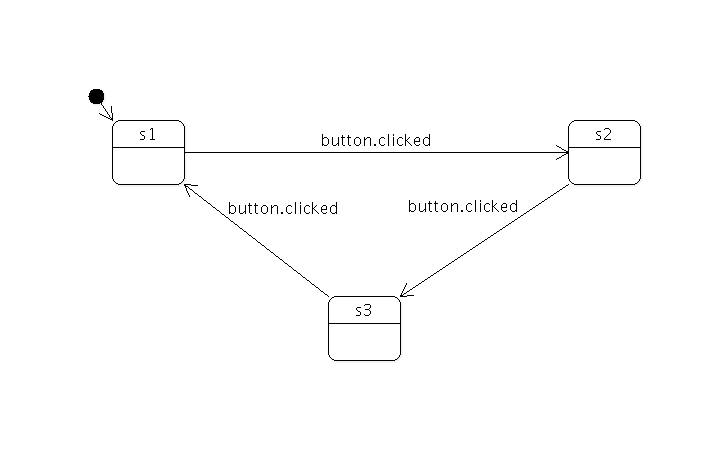
\includegraphics[width=0.7\textwidth]{Abbildungen/statemachinebutton.png}
    \caption[State Machine Beispiel \newline Quelle: \textit{https://doc.qt.io/qt-5/statemachine-api.html}]{State Machine Beispiel}		
    \label{fig:StateMachineexample}
\end{figure}

Zunächst wird die State Machine und ihre Zustände erzeugt (Listing \ref{lst:SM1}). 

\begin{lstlisting}[frame=single, breaklines=true, numbers=left, stepnumber=2, firstnumber=1, numberstyle = \tiny, caption=State Machine Beispiel Teil 1 ,label=lst:SM1]
    QStateMachine machine;
    QState *s1 = new QState();
    QState *s2 = new QState();
    QState *s3 = new QState();
\end{lstlisting}

Anschließend werden jedem Zustand alle für diesen Zustand vorhandenen Transitionen mit der QState::addTransition() Funktion hinzugefügt (Listing \ref{lst:SM2}). Dabei wird angegeben, bei welchem Event (Signal) die Transition ausgeführt werden soll. Wenn ein Transitionssignal auserhalb des Zustands auftritt wird die Transition nicht ausgeführt. 

\begin{lstlisting}[frame=single, breaklines=true, numbers=left, stepnumber=2, firstnumber=1, numberstyle = \tiny, caption=State Machine Beispiel Teil 2 ,label=lst:SM2]
    s1->addTransition(button, SIGNAL(clicked()), s2);
    s2->addTransition(button, SIGNAL(clicked()), s3);
    s3->addTransition(button, SIGNAL(clicked()), s1);
\end{lstlisting}

Listing \ref{lst:SM3} zeigt, wie anschließend die Zustände dem Zustandsautomaten hinzugefügt werden. Außerdem wird der initiale Zustand gesetzt, der bei Programmstart aktiv sein soll. 

\begin{lstlisting}[frame=single, breaklines=true, numbers=left, stepnumber=2, firstnumber=1, numberstyle = \tiny, caption=State Machine Beispiel Teil 3 ,label=lst:SM3]
    machine.addState(s1);
    machine.addState(s2);
    machine.addState(s3);
    machine.setInitialState(s1);
\end{lstlisting}

Abschließend muss die Zustandsmaschine gestartet werden. Ab diesem Zeitpunkt reagiert der Automat auf die Transitionen und wechselt zwischen den Zuständen. 

\begin{lstlisting}[frame=single, breaklines=true, numbers=left, stepnumber=2, firstnumber=1, numberstyle = \tiny, caption=State Machine Beispiel Teil 4 ,label=lst:SM4]
    machine.start();
\end{lstlisting}

Hauptvorteil der so implementierten Zustandsmaschine ist, dass diese vollkommen aysnchron zum restlichen Programm abläuft- somit müssen keine zusätzlichen Schleifen in Tasks gestartet werden. 

Um Funktionen mit einem Zustand zu verknüpfen kann eine Signal, welches jeder Zustand emittiert genutzt werden. Beim Eingang in einen Zustand wird das Signal entered() emittiert, beim verlassen eines Zustands das Signal exited(). In dieser Arbeit wurde ausschließlich mit dem entered() Signal gearbeitet, da dies die Anforderungen ausreichend erfüllt hat. 

Das aufgezeigte Beispiel und weitergehende Erklärungen zu State Machines und den weiteren Klassen sind in \cite{qt_statemachine} zu finden. Darunter sind auch Konzepte zu finden, die ermöglichen Eigenschaften direkt an einen Zustand zu binden. 

\subsection{QListWidget}
\label{sec:QListWidgetItem}

Das QListWidget ermöglicht es, selbst programmierte QListWidgetItems in einer Liste zu organisieren und darzustellen. Zusätzlich werden diverse Funktionen bereitgestellt, mit denen sich die QListWidgetItems ordnen, ergänzen oder finden lassen (vgl. \cite{qt_listwidget}). 

Über die Auswahl der allgemeinen Widgets kann das QListWidget im Layout-Manager ausgewählt werden. 
